\PassOptionsToPackage{dvipsnames}{xcolor}
\documentclass{beamer}

\usepackage[scale=2]{ccicons}
\usepackage{graphicx}
\usepackage{booktabs}
\usepackage{gensymb}
\usepackage{multimedia}
\usepackage{hyperref}
\usepackage{txfonts}

% Beamer configuration
\usetheme[sectionpage=progressbar, numbering=counter, progressbar=frametitle]{metropolis}

\usepackage{pgfplots}
\usepackage{pgfplotsthemetol}

% Progressbar
\setbeamercolor{progress bar}{
    fg=TolLightGreen,
    bg=TolLightGreen!50!black!30
}
\makeatletter
    \setlength{\metropolis@titleseparator@linewidth}{2pt}
    \setlength{\metropolis@progressonsectionpage@linewidth}{2pt}
    \setlength{\metropolis@progressinheadfoot@linewidth}{2pt}
\makeatother

% Footer
\setbeamertemplate{frame footer}{Quentin Brateau, ENSTA Bretagne}

% Block fill
\metroset{block=fill}

\title{Torpedo-like AUV control in constrained environment}
\date{\today}
\author{Quentin Brateau}
\institute{ENSTA Bretagne}

\titlegraphic{
    \centering
    \begin{tabular}{lllll}
        \href{https://www.defense.gouv.fr/aid}{
\includegraphics[height=0.6cm]{imgs/logo_aid}} &
        \href{https://www.gdr-robotique.org/}{
\includegraphics[height=0.6cm]{imgs/logo_gdr}} &
        \href{https://www.ensta-bretagne.fr/fr/}{
\includegraphics[height=0.6cm]{imgs/logo_ensta}} &
        \href{https://labsticc.fr/fr}{
\includegraphics[height=0.6cm]{imgs/logo_labsticc}} &
        \href{https://www.ensta-bretagne.fr/robex/}{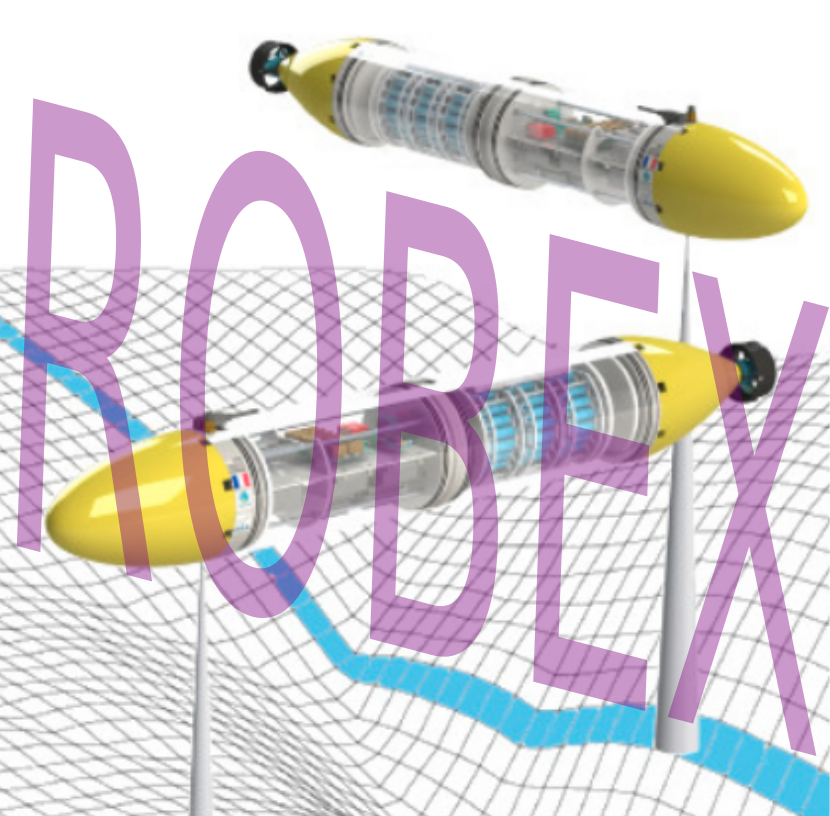
\includegraphics[height=0.6cm]{imgs/logo_robex}}
    \end{tabular}
}

\addtobeamertemplate{frametitle}{}{%
    \begin{tikzpicture}[remember picture,overlay]
    \node[anchor=north east,yshift=2pt] at (current page.north east) {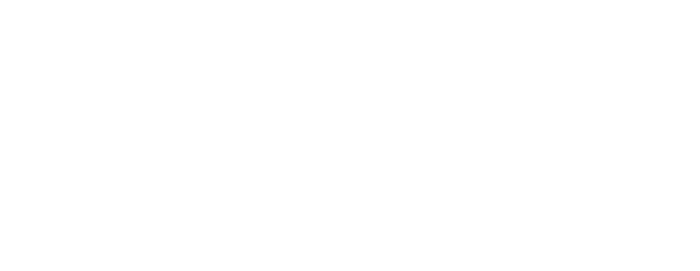
\includegraphics[height=0.9cm]{imgs/logo_ensta_bw}};
    \end{tikzpicture}
}

\begin{document}

    \maketitle

    \section{Introduction}

        \begin{frame}{Introduction}
            \begin{minipage}{0.45\textwidth}
                \begin{block}{AUV}
                    \vspace{0.25cm}
                    \begin{itemize}
                        \item Riptide's micro-uuv \\ 
                        \item Riptide's micro-uuv
                    \end{itemize}
                \end{block}
                \begin{block}{Environment}
                    \begin{itemize}
                        \item Constrained environment \\ 
                        \item Pool, harbor, ...
                    \end{itemize}
                \end{block}
            \end{minipage}
            \hfill
            \begin{minipage}{0.45\textwidth}
                
            \end{minipage}
        \end{frame}

        \begin{frame}{Table of contents}
            \setbeamertemplate{section in toc}[sections numbered]
            \tableofcontents[hideallsubsections]
          \end{frame}
    
    \section{Modeling}

        \begin{frame}{Torpedo model}
            \centering
            \begin{minipage}{0.7\textwidth}
                \begin{block}{Torpedo assumptions}
                    The following statements are equivalent
                    \begin{itemize}
                        \item No side slip effect \\
                        \item No lateral speed
                        \item Velocity along the $\mathnormal{x}$ axis \\
                    \end{itemize}
                \end{block}
                \begin{block}{Torpedo velocity}
                    \begin{equation}
                        \mathbf{v_r} = (v_r, 0, 0)^T
                    \end{equation}
                \end{block}
            \end{minipage}
        \end{frame}

        \begin{frame}{State Equation}
            \centering
            \begin{minipage}{0.7\textwidth}
                \begin{block}{AUV state}
                    The state of the AUV is denoted by $\mathbf{X} = (\mathbf{p}, \mathbf{v_r}, \mathbf{R})$, where:
                    \begin{itemize}
                        \item $\mathbf{p}$ is the position of the AUV \\
                        \item $\mathbf{v_r}$ is the velocity of the AUV in its frame \\
                        \item $\mathbf{R}$ is the rotation matrix between the world and the AUV \\
                    \end{itemize}
                \end{block}
                \begin{block}{State Equation}
                    \begin{eqnarray}
                        \left\{
                            \begin{array}{rcl}
                                \dot{\mathbf{p}} & = & \mathbf{R} \cdot \mathbf{v_r} \\
                                \dot{\mathbf{R}} & = & \mathbf{R} \cdot (\mathbf{\omega_r} \wedge) \\
                                \dot{\mathbf{v_r}} & = & \mathbf{R}^T \cdot g(\mathbf{p}) + \mathbf{a_r}
                            \end{array}
                        \right.
                    \end{eqnarray}
                \end{block}
            \end{minipage}
        \end{frame}

        \begin{frame}{Inputs}
            \centering
            \begin{minipage}{0.7\textwidth}
                \begin{block}{Inputs}
                    \centering
                    Input vector of the system is $\mathbf{u} = (u_0, u_1, u_2, u_3)^T$, where:
                    \begin{itemize}
                        \item $u_0$: thruster velocity \\
                        \item $u_1, u_2, u_3$: fin angles
                    \end{itemize}
                \end{block}
            \end{minipage}
        \end{frame}

        \begin{frame}{Linear acceleration}
            \centering
            \begin{minipage}{0.7\textwidth}
                \begin{block}{Assumptions}
                    \vspace{0.2cm}
                    \begin{itemize}
                        \item Quadratic thrust with velocity
                        \item Quadratic drag with velocity
                    \end{itemize}
                \end{block}
                \begin{block}{Linear acceleration}
                    \begin{equation}
                        \mathbf{a_r} = \underbrace{p_1 \cdot \left(\begin{smallmatrix}u_0 \\ 0 \\ 0 \end{smallmatrix}\right)^2}_{thrust} - \underbrace{p_2 \cdot \mathbf{v_r} \cdot |\mathbf{v_r}|}_{drag}
                    \end{equation}
                \end{block}
            \end{minipage}
        \end{frame}

        \begin{frame}{Angular velocity}
            \centering
            \begin{minipage}{0.8\textwidth}
                \begin{block}{Assumptions}
                    \vspace{0.2cm}
                    \begin{itemize}
                        \item Fin's drag negligible compared to the AUV drag
                        \item Fin's lift used to control the AUV
                        \item Direct response between the fin's angle and the angular velocity
                    \end{itemize}
                \end{block}
                \begin{block}{Angular velocity}
                    \begin{equation}
                        \mathbf{\omega_r} = v_r^{\color{red}{2}} \cdot 
                            \underbrace{
                                \left(
                                \begin{smallmatrix}
                                    -p_3 & -p_3 & -p_3 \\
                                    0 & p_4 \cdot sin(\frac{2\pi}{3}) & -p_4 \cdot sin(\frac{2\pi}{3}) \\
                                    p_4 & p_4 \cdot cos(\frac{2\pi}{3}) & p_4 \cdot cos(\frac{2\pi}{3})
                                \end{smallmatrix}
                                \right)
                            }_{\mathbf{B}(p_3, p_4)} \cdot \left(\begin{smallmatrix}u_1\\ u_2\\ u_3\end{smallmatrix}\right)
                    \end{equation}
                \end{block}
            \end{minipage}
        \end{frame}

    \section{Control}

        \begin{frame}{Control}
            \centering
            \begin{minipage}{0.7\textwidth}
                \begin{block}{Control inputs}
                    \centering
                    Controlled physical quantites are linear acceleration $\mathbf{a_r}$ and angular velocity $\mathbf{\omega_r}$
                \end{block}
                \begin{block}{State Equation}
                    \begin{eqnarray}
                        \left\{
                            \begin{array}{rcl}
                                \dot{\mathbf{p}} & = & \mathbf{R} \cdot \mathbf{v_r} \\
                                \dot{\mathbf{R}} & = & \mathbf{R} \cdot (\mathbf{\omega_r} \wedge) \\
                                \dot{\mathbf{v_r}} & = & \mathbf{R}^T \cdot g(\mathbf{p}) + \mathbf{a_r} - \mathbf{\omega_r} \wedge \mathbf{v_r}
                            \end{array}
                        \right.
                    \end{eqnarray}
                \end{block}
            \end{minipage}
        \end{frame}

        \begin{frame}{Control}
            \centering
            \begin{minipage}{0.7\textwidth}
                \begin{figure}
                    \begin{tikzpicture}
                        \shade[ball color = gray!40, opacity = 0.4] (0,0) circle (2cm);
                        \draw[thick] (0,0) circle (2cm);
                        \draw [thick] (-2,0) arc (180:360:2 and 0.6) coordinate[pos=0.25] (I) coordinate[pos=0.7] (R2);
                        \coordinate (R1) at (0,1.2);
                        \path[thick,ForestGreen,->,>=latex] (R1) edge[bend left] node[pos=0.65,right,ForestGreen] {$\omega_r$} (R2);
                        \node[ForestGreen] at (R1) {$\bullet$} node[ForestGreen] at (R1) [above] {$\mathbf{R}_u$};
                        \node[ForestGreen] at (R2) {$\bullet$} node[ForestGreen] at (R2) [below] {$\mathbf{R}_v$};
                        \node[red] at (I) {$\bullet$} node[red] at (I) [below] {$\mathbf{I}$};
                        \draw[dashed] (2,0) arc (0:180:2 and 0.6);
                    \end{tikzpicture}
                    \caption{$SO(3)$}
                \end{figure}
            \end{minipage}
        \end{frame}

        \begin{frame}{RotUV}
            \centering
            \begin{minipage}{0.3\textwidth}
                \begin{figure}
                    \begin{tikzpicture}
                        \shade[ball color = gray!40, opacity = 0.4] (0,0) circle (2cm);
                        \draw[thick] (0,0) circle (2cm);
                        \coordinate (R1) at (0.5,1.2);
                        \draw [thick] (-2,0) arc (180:360:2 and 0.6) coordinate[pos=0.25] (I) coordinate[pos=0.35] (R2) coordinate[pos=0.7] (R3);
                        \path[thick,ForestGreen,->,>=latex] (R1) edge[bend left=20] node[pos=0.65,right,ForestGreen] {$\omega_r$} (R3);
                        \draw[thick,RoyalPurple,->,>=latex] (0,0) -- node[midway,above left] {$u$} (R1);
                        \draw[thick,RoyalPurple,->,>=latex] (0,0) -- node[midway,above] {$v$} (R2);
                        \node[ForestGreen] at (R1) {$\bullet$} node[ForestGreen] at (R1) [above] {$\mathbf{R}_u$};
                        \node[ForestGreen] at (R2) {$\bullet$} node[ForestGreen] at (R3) [below] {$\mathbf{R}_u^v \cdot \mathbf{R}_u$};
                        \node[red] at (I) {$\bullet$} node[red] at (I) [below] {$I$};
                        \node[ForestGreen] at (R2) {$\bullet$} node[ForestGreen] at (R2) [below] {$\mathbf{R}_v$};
                        \draw[dashed] (2,0) arc (0:180:2 and 0.6);
                    \end{tikzpicture}
                    \caption{$SO(3)$}
                \end{figure}
            \end{minipage}
            \hfill
            \begin{minipage}{0.55\textwidth}
                \begin{block}{Vector to vector formulation}
                    \begin{equation}
                        \begin{array}{rcl}
                            \mathbf{K}_u^v & = & vu^T - uv^T \\
                            \mathbf{R}_u^v & = & \mathbf{I} + \mathbf{K}_u^v + \frac{1}{1 + \langle u, v\rangle} (\mathbf{K}_u^v)^2
                        \end{array}
                    \end{equation}
                \end{block}
            \end{minipage}
        \end{frame}

    \appendix

    \begin{frame}[standout]
        Questions?
    \end{frame}

    \begin{frame}{Repartition matrix}
        \centering
        \begin{minipage}{0.8\textwidth}
            \begin{block}{Fin's lift}
                $\forall i \in \{0, 1, 2\}:$
                \begin{itemize}
                    \item Force $\mathbf{f_i} = \alpha \cdot u_i \cdot v^2 \cdot (0, 1, 0)^T$
                    \item Orientation $\mathbf{R_i} = \mathbf{R_x}\left(\frac{2i\pi}{3}\right)$
                    \item Center of pressure $\mathbf{q_i} = (\mathit{l_x}, 0, \mathit{l_z})^T$
                    \item Torque $\mathbf{\tau_i} = \mathbf{R_i} \cdot \mathbf{q} \wedge \mathbf{f_i}$
                \end{itemize}
            \end{block}
            \begin{block}{Angular velocity}
                \begin{equation}
                    \mathbf{\omega_r} = v_r^2 \cdot 
                        \underbrace{
                            \left(
                            \begin{smallmatrix}
                                -p_3 & -p_3 & -p_3 \\
                                0 & p_4 \cdot sin(\frac{2\pi}{3}) & -p_4 \cdot sin(\frac{2\pi}{3}) \\
                                p_4 & p_4 \cdot cos(\frac{2\pi}{3}) & p_4 \cdot cos(\frac{2\pi}{3})
                            \end{smallmatrix}
                            \right)
                        }_{\mathbf{B}(p_3, p_4)} \cdot \left(\begin{smallmatrix}u_1\\ u_2\\ u_3\end{smallmatrix}\right)
                \end{equation}
            \end{block}
        \end{minipage}
    \end{frame}
    
\end{document}